\documentclass[aspectratio=169,10pt]{beamer}
\usetheme{Boadilla}
\usepackage{booktabs,graphicx,amsmath}
\usepackage{tikz}
\usetikzlibrary{arrows.meta,calc}
\definecolor{navy}{HTML}{17365D}
\setbeamercolor{structure}{fg=navy}
\setbeamercolor{frametitle}{fg=navy}
\setbeamertemplate{navigation symbols}{}
\setbeamertemplate{footline}[frame number]
\graphicspath{{figures/}}
\title[Photon pointing v4]{Calorimeter pointing: v4 Stage 1 preparation}
\subtitle{Stored inputs, offline smearing and the bounded signal check}
\author{FCC-ee $\Lambda_b\to\Lambda\gamma$ study}
\date{5 October 2026}
\begin{document}
\begin{frame}\titlepage
\vspace{-0.4cm}\centering\small PI checkpoint: prepare reproducible Zbb, Zcc, Zss and 100k forced-mode reprocessing.
\end{frame}

\begin{frame}{Pointing study: four steps}
\small
\begin{columns}[T,onlytextwidth]
\column{0.23\textwidth}
\begin{block}{1. Save the photon}
\centering
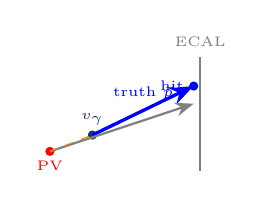
\begin{tikzpicture}[scale=.83,>=Stealth]
 \draw[gray,thick] (2.55,0.15)--(2.55,1.9) node[above,font=\tiny]{ECAL};
 \fill[red] (.25,.45) circle (2pt) node[below,font=\tiny]{PV};
 \fill[navy] (.9,.7) circle (2pt) node[above,font=\tiny]{$v_\gamma$};
 \draw[blue,very thick,-{Stealth}] (.9,.7)--(2.45,1.45) node[midway,above,font=\tiny]{truth $\vec p$};
 \draw[gray,thick,-{Stealth}] (.25,.45)--(2.45,1.18);
 \draw[orange,dashed] (.25,.45)--(.9,.7);
 \fill[blue] (2.45,1.45) circle (2pt) node[left,font=\tiny]{hit};
\end{tikzpicture}\par
\raggedright\scriptsize Keep $E_{reco},\vec p_{reco}$, matched truth $\vec p_\gamma$ and production point. Reco direction currently assumes the photon starts at the origin.
\end{block}
\column{0.23\textwidth}
\begin{block}{2. Predict both hits}
\centering
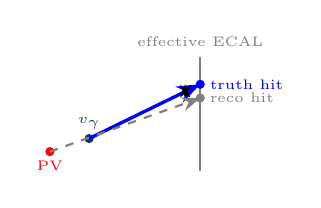
\begin{tikzpicture}[scale=.83,>=Stealth]
 \draw[gray,thick] (2.55,0.15)--(2.55,1.9) node[above,font=\tiny]{effective ECAL};
 \fill[red] (.25,.45) circle (2pt) node[below,font=\tiny]{PV};
 \fill[navy] (.85,.65) circle (2pt) node[above,font=\tiny]{$v_\gamma$};
 \draw[blue,very thick,-{Stealth}] (.85,.65)--(2.55,1.48);
 \draw[gray,dashed,thick,-{Stealth}] (.25,.45)--(2.55,1.27);
 \fill[blue] (2.55,1.48) circle (2pt) node[right,font=\tiny]{truth hit};
 \fill[gray] (2.55,1.27) circle (2pt) node[right,font=\tiny]{reco hit};
 \draw[<->] (2.32,1.27)--(2.32,1.48);
\end{tikzpicture}\par
\raggedright\scriptsize Intersect the truth ray from $v_\gamma$ with the cylinder/endcap. Also save the origin-based reco projection as a position-response comparison.
\end{block}
\column{0.23\textwidth}
\begin{block}{3. Smear the direction}
\centering
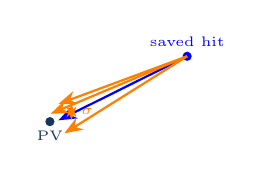
\begin{tikzpicture}[scale=.83,>=Stealth]
 \fill[navy] (.35,.45) circle (2pt) node[below,font=\tiny]{PV};
 \fill[blue] (2.45,1.45) circle (2pt) node[above,font=\tiny]{saved hit};
 \draw[blue,thick,-{Stealth}] (2.45,1.45)--(.48,.47);
 \draw[orange,thick,-{Stealth}] (2.45,1.45)--(.48,.72);
 \draw[orange,thick,-{Stealth}] (2.45,1.45)--(.57,.27);
 \draw[orange,thick,-{Stealth}] (2.45,1.45)--(.36,.57);
 \draw[<->,orange] (.68,.48)--(.68,.72) node[midway,right,font=\tiny]{$\sigma$};
\end{tikzpicture}\par
\raggedright\scriptsize Add two Gaussian angular components in the tangent plane. Scan $\sigma=0.5,0.7,0.9,1.1,1.3,1.5$ mrad. Same photon, same random draw across candidates.
\end{block}
\column{0.23\textwidth}
\begin{block}{4. Measure after BDT}
\centering
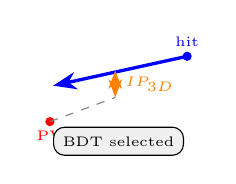
\begin{tikzpicture}[scale=.83,>=Stealth]
 \fill[red] (.3,.45) circle (2pt) node[below,font=\tiny]{PV};
 \draw[blue,very thick,-{Stealth}] (2.4,1.45)--(.35,1.0);
 \fill[blue] (2.4,1.45) circle (2pt) node[above,font=\tiny]{hit};
 \draw[gray,dashed] (.3,.45)--(1.3,.82);
 \draw[<->,orange,thick] (1.3,.82)--(1.3,1.23) node[midway,right,font=\tiny]{$IP_{3D}$};
 \node[draw,rounded corners,fill=gray!12,font=\tiny] at (1.35,.15){BDT selected};
\end{tikzpicture}\par
\raggedright\scriptsize Set $\vec p^{hyp}=E_{reco}\hat n_{smear}$. Compute $IP_{3D}$ and $|d_0|$ to the reconstructed PV; scan cuts and signal/background efficiencies offline.
\end{block}
\end{columns}
\vspace{0.12cm}
\centering\scriptsize The truth-hit picture assumes an ideal hit position; the reco-hit picture inherits current position uncertainty. Neither assigns a pointing significance without a covariance model.
\end{frame}

\begin{frame}{What is stored and how pointing hypotheses are made}
\begin{columns}[T]
\begin{column}{0.54\textwidth}
For each reconstructed $\Lambda_b$ candidate the v4 tuple keeps:
\begin{itemize}
\item measured photon $E_{\rm reco},(p_x,p_y,p_z)_{\rm reco}$ and reco index;
\item matched truth photon $(p_x,p_y,p_z,E)$ and production vertex;
\item predicted ECAL hit from the displaced truth ray and, separately, from the current origin-based reco direction;
\item reconstructed PV and effective surface parameters.
\end{itemize}
Smear the truth direction in two orthogonal tangent directions with Gaussian component width $\sigma=0.5$–$1.5$ mrad (six points), then set $\vec p_{\gamma}^{\,hyp}=E_{\rm reco}\hat n_{\rm smear}$. Reuse the same random draw for a photon shared by candidates. Evaluate $IP_{3D}=|(\vec x_{hit}-\vec x_{PV})\times\hat n|$ and $|d_0|$ offline after BDT.
\end{column}
\begin{column}{0.43\textwidth}
\centering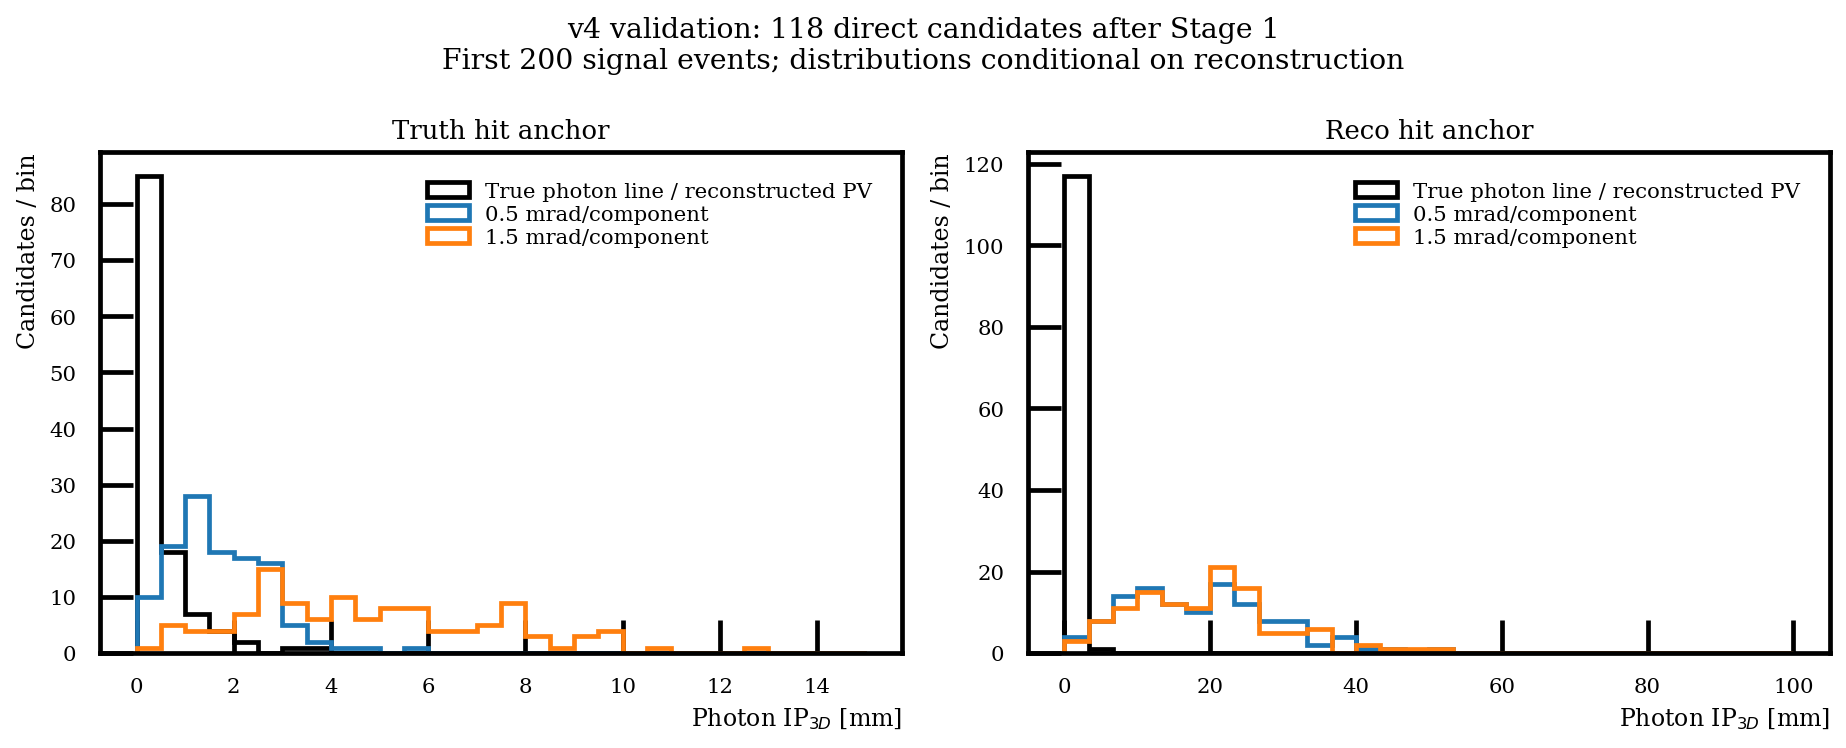
\includegraphics[width=\linewidth]{stage1_v4_pointing_validation.png}
\scriptsize 118 matched direct candidates from the first 200 signal input events. Conditional shapes, not yields. Truth-hit anchor assumes ideal position; reco anchor inherits current position uncertainty.
\end{column}
\end{columns}
\vspace{0.1cm}\tiny Effective IDEA geometry: barrel $R=2250$ mm, $|z|=2500$ mm; endcap inner radius inferred as $2500/\sinh(3)$. A pointing significance needs a position/direction covariance not yet modelled.
\end{frame}

\begin{frame}{What the 200-event signal check established}
\small
\begin{center}
\begin{tabular}{lr@{\qquad}lr}
\toprule
Input events & 200 & Candidate-bearing events & 121\\
Candidates & 133 & Direct / wrong combinations & 118 / 15\\
Old branches identical & 474 / 474 & Pointing vectors valid & 28 / 28\\
Stage 2 audit / selected & 133 / 129 & After frozen BDT cut & 46\\
\bottomrule
\end{tabular}
\end{center}
\vspace{0.25cm}
\begin{columns}[T,onlytextwidth]
\begin{column}{0.48\textwidth}
\begin{block}{What passed}
The true-ray projection closes to its saved hit. The new fields survive Stage 2 preparation and the frozen BDT score. The paired run kept the same 121 output events and the same 133 candidates.
\end{block}
\end{column}\hfill
\begin{column}{0.48\textwidth}
\begin{block}{What remains to measure}
Full signal and Zss/Zcc processing must establish unresolved fractions, pointing-cut efficiencies, mass and angle sculpting, and signal acceptance. This small signal check does not measure flavour rejection.
\end{block}
\end{column}
\end{columns}
\vspace{0.15cm}
\begin{block}{v4 Condor check only}
Zbb: 4,398 files; Zcc: 5,018; Zss: 5,015. Each has 1,200 chunks, four cores/job, accounting group \texttt{group\_u\_FCC.local\_gen} and \texttt{workday} flavour. All three checks passed; no jobs were submitted.
\end{block}
\end{frame}

\begin{frame}{100k Stage 1 rerun: available modes and next commands}
\small
\begin{tabular}{lll}
\toprule
Mode & Current merged input & Status\\
\midrule
$\Lambda\gamma$ PHSP & \texttt{Lb2LambdaGamma\_nev100000...root} & ready\\
$\Lambda\gamma$ HELAMP & \texttt{Lb2LambdaGammaPhysics\_nev100000...root} & ready\\
$\Lambda\eta$ PHSP / HELAMP & \texttt{Lb2LambdaEta(Physics)\_nev100000...root} & ready\\
$\Lambda\pi^0$ HELAMP & \texttt{Lb2LambdaPi0Physics\_nev100000...root} & ready\\
$\Lambda\pi^0$ PHSP & \texttt{Lb2LambdaPi0\_nev100000...root} & merged file not found\\
\bottomrule
\end{tabular}
\vspace{0.4cm}
\begin{enumerate}
\item Run \texttt{scripts/run\_stage1\_v4\_forced\_100k.sh --check-only}; it lists exact inputs/outputs. Then use \texttt{--run} to process available modes. Default uses four concurrent samples × eight CPUs (32 cores); tune \texttt{V4\_DIRECT\_JOBS} and \texttt{V4\_DIRECT\_CPUS}. Each output gets a v4 tuple validation JSON.
\item Generate/merge the missing $\pi^0$ PHSP 100k sample using seed base 72001 from \texttt{config/config.yaml}, then rerun the checker.
\item After review, submit Z flavours with \texttt{scripts/submit\_stage1\_v4\_zflavours.sh --submit}; default is \texttt{--check-only}.
\end{enumerate}
\tiny Production commands, output paths, file inventory and check logs are recorded in the v4 howto and frozen job preparation note. No full 100k or Condor production was launched here.
\end{frame}
\end{document}
